\section{Structures de données}

    \subsection{XML}
        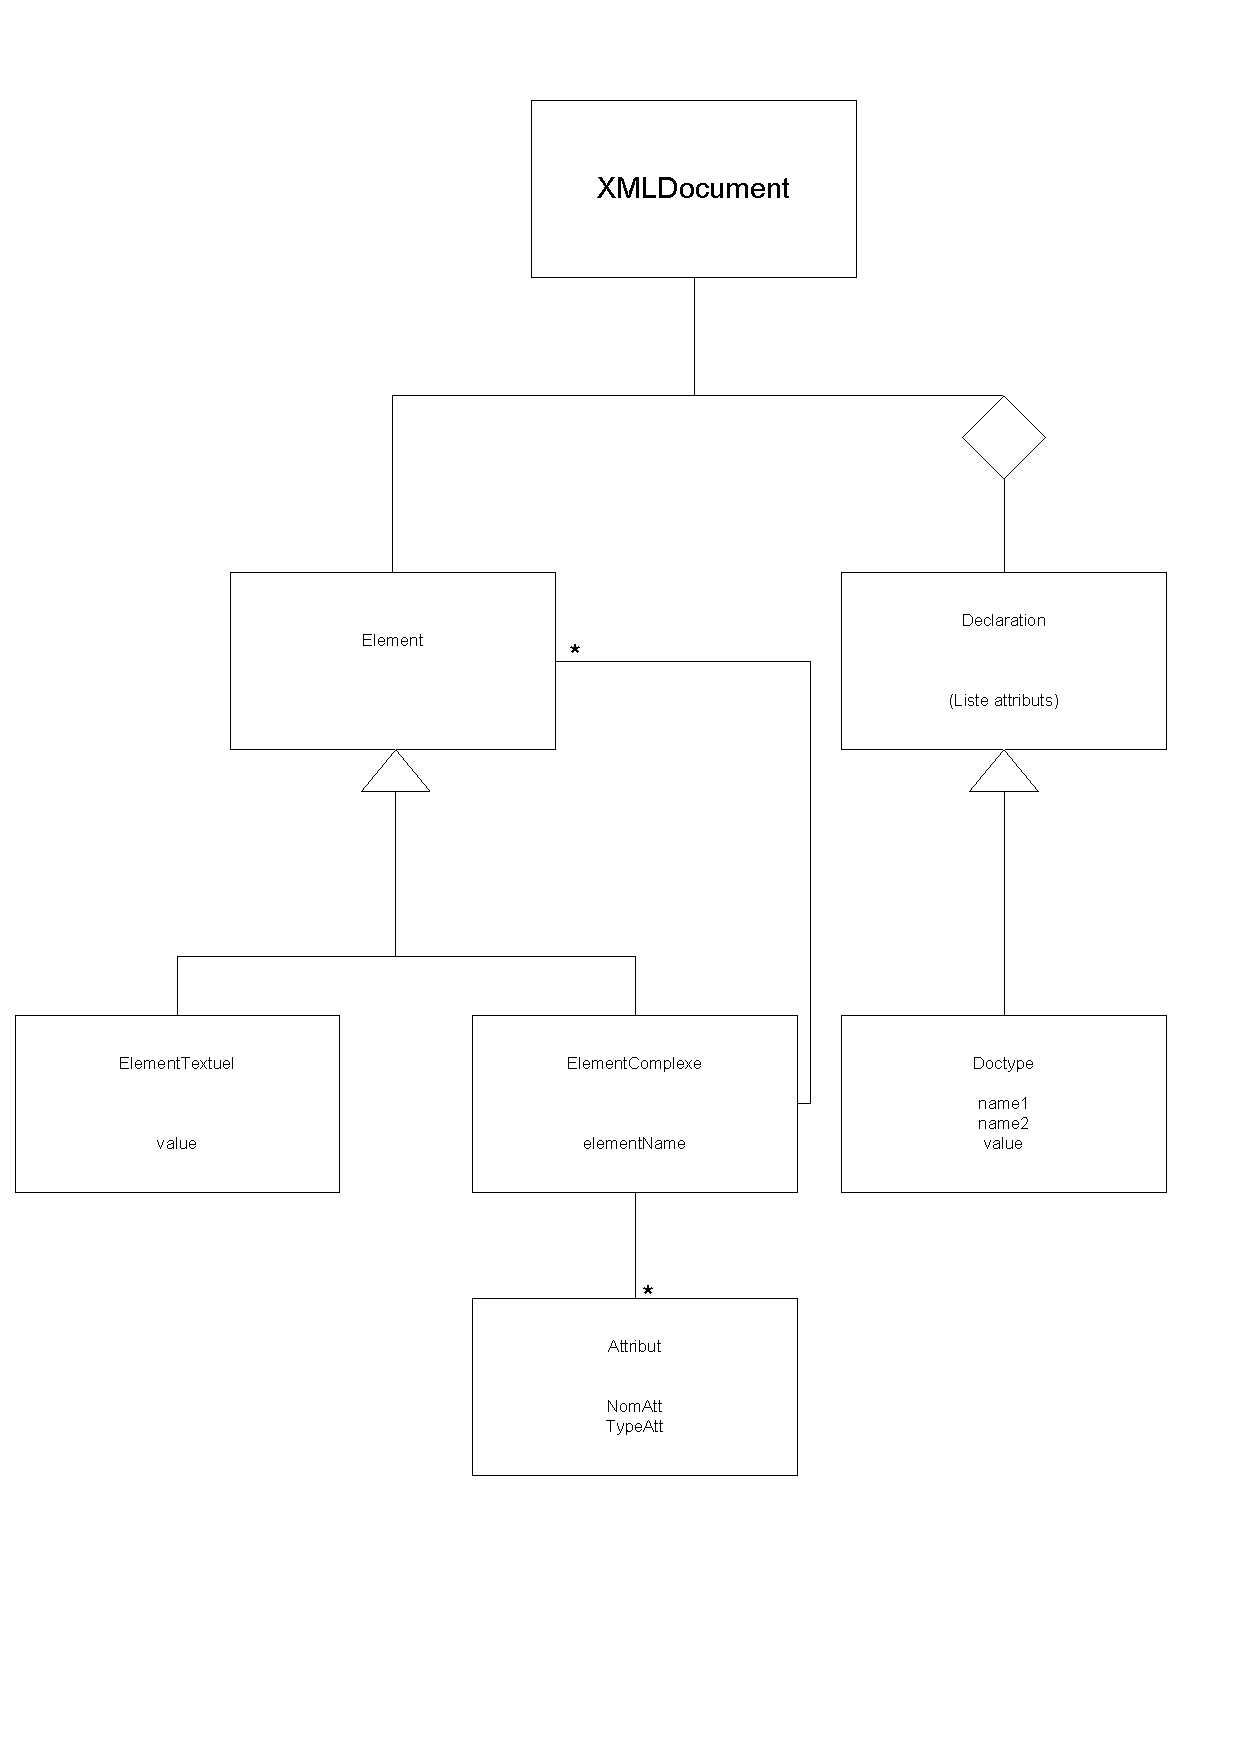
\includegraphics[width=0.7\textwidth]{img/ClassesXML.pdf}\\
        La structure de donnée généré pendant la lecture du XML
        
    \subsection{DTD}
        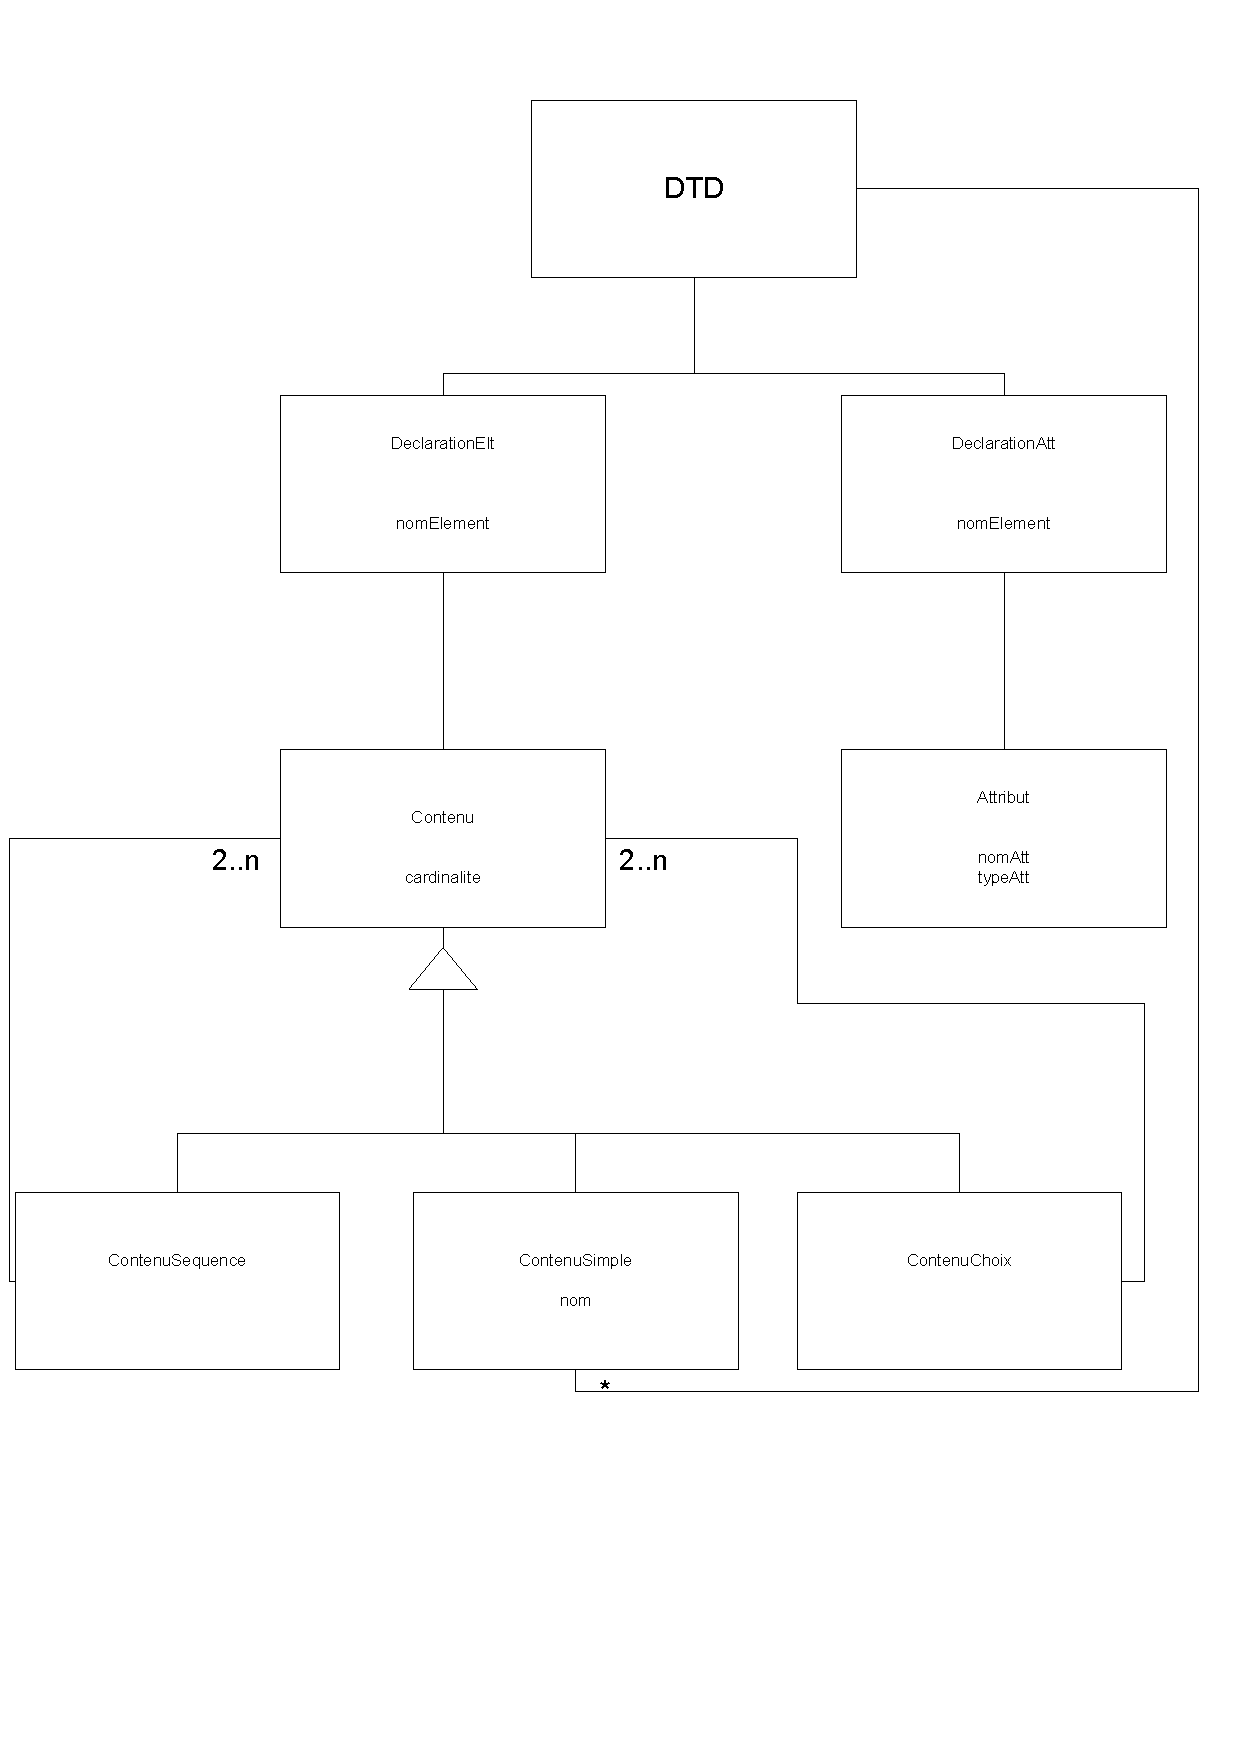
\includegraphics[width=0.7\textwidth]{img/ClassesDTD.pdf}\\
        La structure de donnée généré pendant la lecture de la DTD
        
\section{Algorithmes}

    \subsection{Validation}
	
	\begin{algorithm}
	\caption{validateXML(XML $xml$, DTD $dtd$)}
	\begin{algorithmic}
	    \STATE String $exp \gets$ transformXML(xml) \COMMENT{transformer le fichier XML en une expression a valider}
	    \STATE String $pattern \gets$ transformDTD(dtd) \COMMENT{transformer le fichier DTD en pattern}
	    \STATE bool $resultat \gets$ match(exp, pattern) \COMMENT{valider}
    \end{algorithmic}
    \end{algorithm}
    
    \begin{algorithm}
	\caption{transformDTD(DTD dtd)}
    \begin{algorithmic}
	    \RETURN tranformDeclarationElement(dtd.racine) \COMMENT{on commencer par l'element racine}
    \end{algorithmic}
    \end{algorithm}
        
    \begin{algorithm}
	\caption{tranformDeclarationElement(DeclarationElement decEle)}    
    \begin{algorithmic}
	    \STATE String $result$ \COMMENT{transformer recursivement} 
        \IF{$decEle$ est textuel}
		    \STATE $result \gets$ "\textless"+decEle.nom+decATTLIST"\textgreater decText"\textless/"+decEle.nom+"\textgreater
	    \ELSE
		    \STATE $result \gets$ "(\textless"+decEle.nom+decATTLIST"\textgreater"
		    \FOR{chaque element fils $filsEle$}
			    \IF{\NOT getCardinalité()}
				    \STATE $result$ += tranformDeclarationElement(filsEle)
			    \ELSE
				    \STATE $result$ += "(" tranformDeclarationElement(filsEle)+cardinalite(filsEle)+")"
		        \ENDIF
	        \ENDFOR
	    \ENDIF
	\end{algorithmic}
    \end{algorithm}
        
    \subsection{Transformation}
        %TODO ici l'algo fait par Baptiste
